\section{Glioma Segmentation with Cascaded Unet}

\subsection*{Ссылка} \url{https://arxiv.org/abs/1810.04008}
\subsection*{Введение}
Точная сегментация и реконструкция медицинских 3D изображений способны дать 
больше необходимой информации о прогрессировании заболевания и позволяют терапевту 
спланировать успешный курс лечения для больного. В данной работе авторы представляют
каскадный вариант популярной сети UNet, который итеративно улучшает результаты сегментации, 
полученные на предыдущих шагах. 
\subsection*{Основная идея}
Предложенный метод может быть представлен как цепь классификаторов 
\(C_i\), одинаковой топологии F, у каждого из которых свой собственный 
набор параметров \(W_i\) для оптимизации в течение обучения.
Результат вычисления \(i\)-го шага представляется следующим образом: 
\(Y_i=F(X_i,Y_{i-1}, Y_{i-2}, W_i)\). Каждый из базовых блоков \(C_i\) - это
сеть архитектуры UNet, измененная для задачи сегментации глиом. В сравнении 
со стандартной архитектурой UNet, в предложенной модели используется несколько 
энкодеров, которые раздельно обрабатывают входные данные. Также, предложен метод объединения 
их выхода: в UNet \(i\)-й выход декодера зависит от выхода соответствующего 
энкодера и выхода предыдущего декодера - \(d_i^{t}=f(e_i^{t}, d^{t}_{i-1})\). 
Раскрывая первую свертку \(f\), получаем - \(d_i^{t}=g(W_{i,e}^{t}e_i^{t}+W_{i},d^{t}d^{t}_{i-1})\).
Далее предлагается объединить контекст, полученный на более низких слоях, 
добавляя соответствующий выход \(y^t\), поэтому \(d_i^{t}=g(W_{i,e}^{t}e_i^{t}+W_{i,d}^{t}d^{t}_{i-1}+W_{i,y}^{t}y^{t-i})\).
\\
\begin{minipage}{1.0\linewidth}
    \begin{center}
        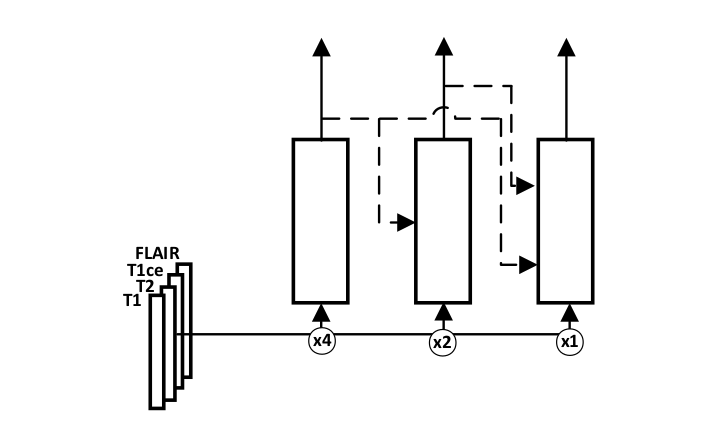
\includegraphics[scale=0.6]{ann7_arch.png}
        \caption{Схематическое представление метода, описанного в статье.
        T1, T2, T1ce, FLAIR - входные модальности МРТ-изображения, x4,x2 - понижающий
        фактор входа сети. Пунткирные линии - соединения между блоками \(C_i\).}
    \end{center}
\end{minipage}


\subsection*{Данные}
BraTS 2018
\subsection*{Результаты}
Результат сегментации  оценивался по метрике Dice, отдельно вычисленной
для следующих частей опухоли: WT (whole tumor) -  вся опухоль, ET (enchancing tumor) - 
усиливающаяся часть опухоли и TC (tumor core) - ядро опухоли. \\
Результаты без аугментации выходов: \\
\begin{minipage}{1.0\linewidth}
    \begin{center}
        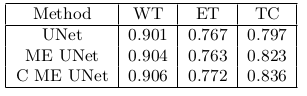
\includegraphics[scale=0.8]{ann7_res.png}
    \end{center}
\end{minipage}
Результаты с аугментацией выходов: \\
\begin{minipage}{1.0\linewidth}
    \begin{center}
        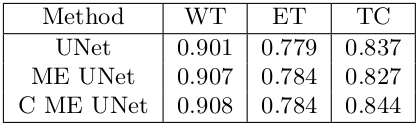
\includegraphics[scale=0.6]{ann7_res1.png}
    \end{center}
\end{minipage}
\subsection*{Заключение}
В данной работе был предложен алгоритм автоматической сегментации 
опухолей головного мозга по МРТ-зображениям, который решает также проблему
мультимодального входа и показывает хорошие резльтаты по сравнению с моделью UNet.


